%% nicht vergessen draft raus zu nehmen, um echte Bilder einzubinden und die Problem-Vierecke verschwinden zu lassen
\documentclass[11pt,a4paper,oneside,svgnames]{report}

\usepackage[utf8]{inputenc}
\usepackage[T1]{fontenc}
\usepackage{lmodern}
\usepackage{eurosym}
\usepackage[british]{babel}

\usepackage{ae}
\usepackage{hyperref}
\usepackage{float}
\usepackage[table]{xcolor}
\usepackage{colortbl}
\usepackage{multirow}
\usepackage{tabularx}
\usepackage{graphicx}
\usepackage{tikz}
\usepackage{kpfonts}
\usepackage[explicit]{titlesec}
\usepackage[acronym,nonumberlist,style=tree]{glossaries}
\usepackage{amssymb}
\usepackage[left=3.65cm,right=3.65cm,top=3cm,bottom=3cm]{geometry}


%BEGIN Chapter Definition

\makeatletter
\def\thickhrulefill{\leavevmode \leaders \hrule height 1ex \hfill \kern \z@}
\def\@makechapterhead#1{%
  \vspace*{0\p@}%
  {\parindent \z@ \raggedleft \reset@font
            \scshape \@chapapp{} \thechapter
        \par\nobreak
        \interlinepenalty\@M
    \Huge \bfseries #1\par\nobreak
    %\vspace*{1\p@}%
    \hrulefill
    \par\nobreak
    \vskip 20\p@
  }}
\def\@makeschapterhead#1{%
  \vspace*{0\p@}%
  {\parindent \z@ \raggedleft \reset@font
            \scshape \vphantom{\@chapapp{} \thechapter}
        \par\nobreak
        \interlinepenalty\@M
    \Huge \bfseries #1\par\nobreak
    %\vspace*{1\p@}%
    \hrulefill
    \par\nobreak
    \vskip 20\p@
  }}

%END Chapter Definition

%BEGIN Title Definition

\makeatletter
\def\thickhrulefill{\leavevmode \leaders \hrule height 1pt\hfill \kern \z@}
\renewcommand{\maketitle}{\begin{titlepage}%
    \let\footnotesize\small
    \let\footnoterule\relax
    \parindent \z@
    \reset@font
    \null\vfil
    \begin{flushleft}
      \huge \@title
    \end{flushleft}
    \par
    \hrule height 4pt
    \par
    \begin{flushright}
      \LARGE \@author \par
    \end{flushright}
    \vskip 60\p@
    \vfil\null
  \end{titlepage}%
  \setcounter{footnote}{0}%
}

%END Title Definition

%Verschissener rotierter Text für verschissene Tabelle 14.1/2
\makeatletter
\newsavebox\zzz
\def\mystrut{%
\dimen@\wd\zzz
\divide\dimen@\thr@@
\advance\dimen@-\dp\@arstrutbox
\rule\z@\dimen@}

\def\rotatezzz{%
\rotatebox{90}{\rlap{\kern-\dp\@arstrutbox\usebox\zzz}}}
%END Verschissener rotierter Text

\makeatother
\title{Software Requirements Specifications for Project ``BookExpress''}
\author{Marc A. Harnos\\ {mharnos@gmail.com} \and Joscha Rapp\\ {jraxxo@gmail.com} \and Christian Schulz\\ {crs.s@gmx.net}}
\author{Marc A. Harnos\\ Joscha Rapp\\ Christian Schulz}
\date{October 2012}

\definecolor{tableHead}{HTML}{5393B7}
\definecolor{tableEven}{HTML}{DAF1FF}
\definecolor{tableOdd}{HTML}{ADD0E5}
\definecolor{tableFoot}{HTML}{5393B7}

\definecolor{linkcolour}{rgb}{0,0.2,0.6}

\hypersetup{colorlinks,breaklinks,urlcolor=linkcolour,linkcolor=linkcolour}
\renewcommand{\arraystretch}{1.25}

\makeglossaries

\newglossaryentry{pin}{name=PIN,description={Personal Identification Number},plural=PINs, first={Personal Identification Number (PIN)}}

\newacronym{led}{LED}{light-emitting diode}
\newacronym{html}{HTML}{Hypertext Markup Language}
\newacronym{css}{CSS}{Cascade Stylesheet}
\newacronym{js}{JS}{JavaScript}
\newacronym{ie}{IE}{InternetExplorer}
\newacronym{vm}{VM}{Virtual Machine}
\newacronym{ide}{IDE}{Integrated Development Environment}


\begin{document}

\maketitle
\tableofcontents

\chapter*{Document History}

\begin{table}[H]
\centering
\begin{tabular}{|l|l|l|l|}
\hline 
Editor(s) & Date & Purpose of Editing & Version \\ 
\hline 
Harnos, Rapp, Schulz & 2012-10-01 & Initial Document Creation & v0.01 \\ 
\hline
Harnos, Rapp & 2012-10-08 & Fick Das & v0.02 \\ 
\hline
Schulz & 2012-10-08 & Fick Das Nicht - Überstimmt & v0.03 \\ 
\hline 
\end{tabular}
\caption{Document History Table}
\label{tab:document-history}
\end{table}


\chapter{Product Purpose}
To handle the addition of new books and the distribution in a better way, "BookExpress" asked us to develop an IT solution to optimize the idle time and labour usage by getting rid of the current, deprecated system. Furthermore one important goal of the software solution is to be very user friendly and easy to use; also there should be remote access implemented, so several customers can access the software at once and distribution partners can access and keep their book stock up to date.
\section{Obligatory Requirements (``must have'')}
\subsection{Communication with Publishers}
The direct connection between the \textbf{publishers} and BookExpress shall be implemented by providing a web interface for the publishers.\\
\begin{itemize}
\item As each publisher also has a \gls{pin}, it will be used as the account name for the interface.
\item The web interface has to provide the following features for the publisher: maintain the book database (add books, remove books, edit book data), edit their personal data, view statistics on how often which books are bought
\item The interface has to be comfortably accessible from mobile devices as well, the data that is transmitted should be minimal\\
\end{itemize}
\subsection{Communication with Customers}
The direct connection between the \textbf{customers} and BookExpress shall also be implemented by providing a web interface for the customers.\\
\begin{itemize}
\item As each customer already has a unique identifier, the PIN, we will use it as an account name for the login.
\item The web interface has to provide the following features: view catalogue and stock, submit orders, view  the current state of their orders and cancel them (if they haven't been shipped yet)
\item The system has to assign a unique ID to each order, ideally incorporating the PIN of the customer
\item The interface has to be comfortably accessible from mobile devices as well, the data that is transmitted should be minimal\\
\end{itemize}
\subsection{Internal Administration}
The employees of BookExpress shall be provided a web interface as well. 
\begin{itemize}
\item Each employee will get a unique user ID to log into the web interface. Ideally, this will be formatted along the lines of surname.name or something similar.
\item The web interface must provide the following features for the employees: processing, editing and cancellation  of submitted orders, directly contact the customers and publishers as well as the truck fleet and the warehouse
\item Furthermore, the underlying system shall generate logfiles with login times, error codes and statistics (e.g. which books are ordered the most and by whom) for the publishers and the accounting and IT department / tech support.
\item The interface has to be comfortably accessible from mobile devices as well, the data that is transmitted should be minimal\\ 
\end{itemize}
\subsection{Support}
\begin{itemize}
\item The system should be as automatic as possible - we need a good, user-oriented manual.
\item Additionally, a context-sensitive help tool has to be implemented in the interface itself. 
\item Moreover, As we want to make sure that the system is as reliable as possible, we will need a dedicated support team that is available 24/7 and can be dispatched in less than 2 hours to fix critical issues.
\end{itemize}

\section{Optional Requirements (``nice to have'')}
\begin{itemize}
\item Book Stores should be able to save recurring orders
\item Book Stores should be notified when the delivery of their order is imminent\\
\end{itemize}

\section{Non-Requirements (``need not have'')}
\begin{itemize}
\item The software should not allow final customers to buy books. It is only intended for retailers.
\item Moreover, invoices are generated elsewhere, as well as financial reports, so the system should not interfere with that.\\
\end{itemize}
\chapter{Product Environment}
The Product takes the orders from the book stores and files them into the system, so that they can be prepared for shipping. For different sized book stores there should be several account types with separate functionality and different options for packaging and ordering. The targeting groups of the software solution are the book store owners(our consumers), the assistants of "BookExpress" and the distribution partners.
\section{Application Area}
The new IT system should replace the old system and provide administrative and commercial functions to relieve the employees of unnecessarily complex administrative tasks. Certain processes can be handled without any interaction at all, e.g. if a book runs low in stock, the system will automatically order new copies from the publisher. 
\section{User Groups}
\begin{itemize}
\item BookExpress commercial employees
\item BookExpress IT employees
\item Publishers
\item Book Stores
\end{itemize}
\section{Operating Conditions}

The hardware and software requirements for each system found in the following table, are just roughly described specifications. For detailed information concerning the product environment see section \ref{sec:tpe}.

\rowcolors{1}{tableEven}{tableOdd}
\begin{table}[H]
\centering
\begin{tabular}{p{2.5cm}p{4.5cm}p{4cm}p{1.5cm}}
\rowcolor{white} \textbf{System} & \textbf{Physical Environment} & \textbf{Supervision} & \textbf{Uptime}\\
\hline
\cellcolor{white} BookExpress & Desktop-PC and Laptops. Mobile Clients at Logistics. & BookExpress IT employees & Business hours\\
\cellcolor{white} Web Interface for Clients & Mostly Desktop-PC and laptops. & Error support by BookExpress IT employees & 24/7\\
\cellcolor{white} Server & Backup system. Isolated server room. & BookExpress IT employees & 24/7\\
\end{tabular}
\caption{Operating Conditions}
\label{tab:opcon}
\end{table}

\chapter{Product Overview}
The following diagram is a graphical representation for specifying the right on accessing the different processes which the program provides.
BookExpress has a restricted rights management with several roles (see {sec:rights-management}) to the defined functions of the product (see \ref{sec:product-functions}).

\begin{figure}[h!]
 \begin{center}
  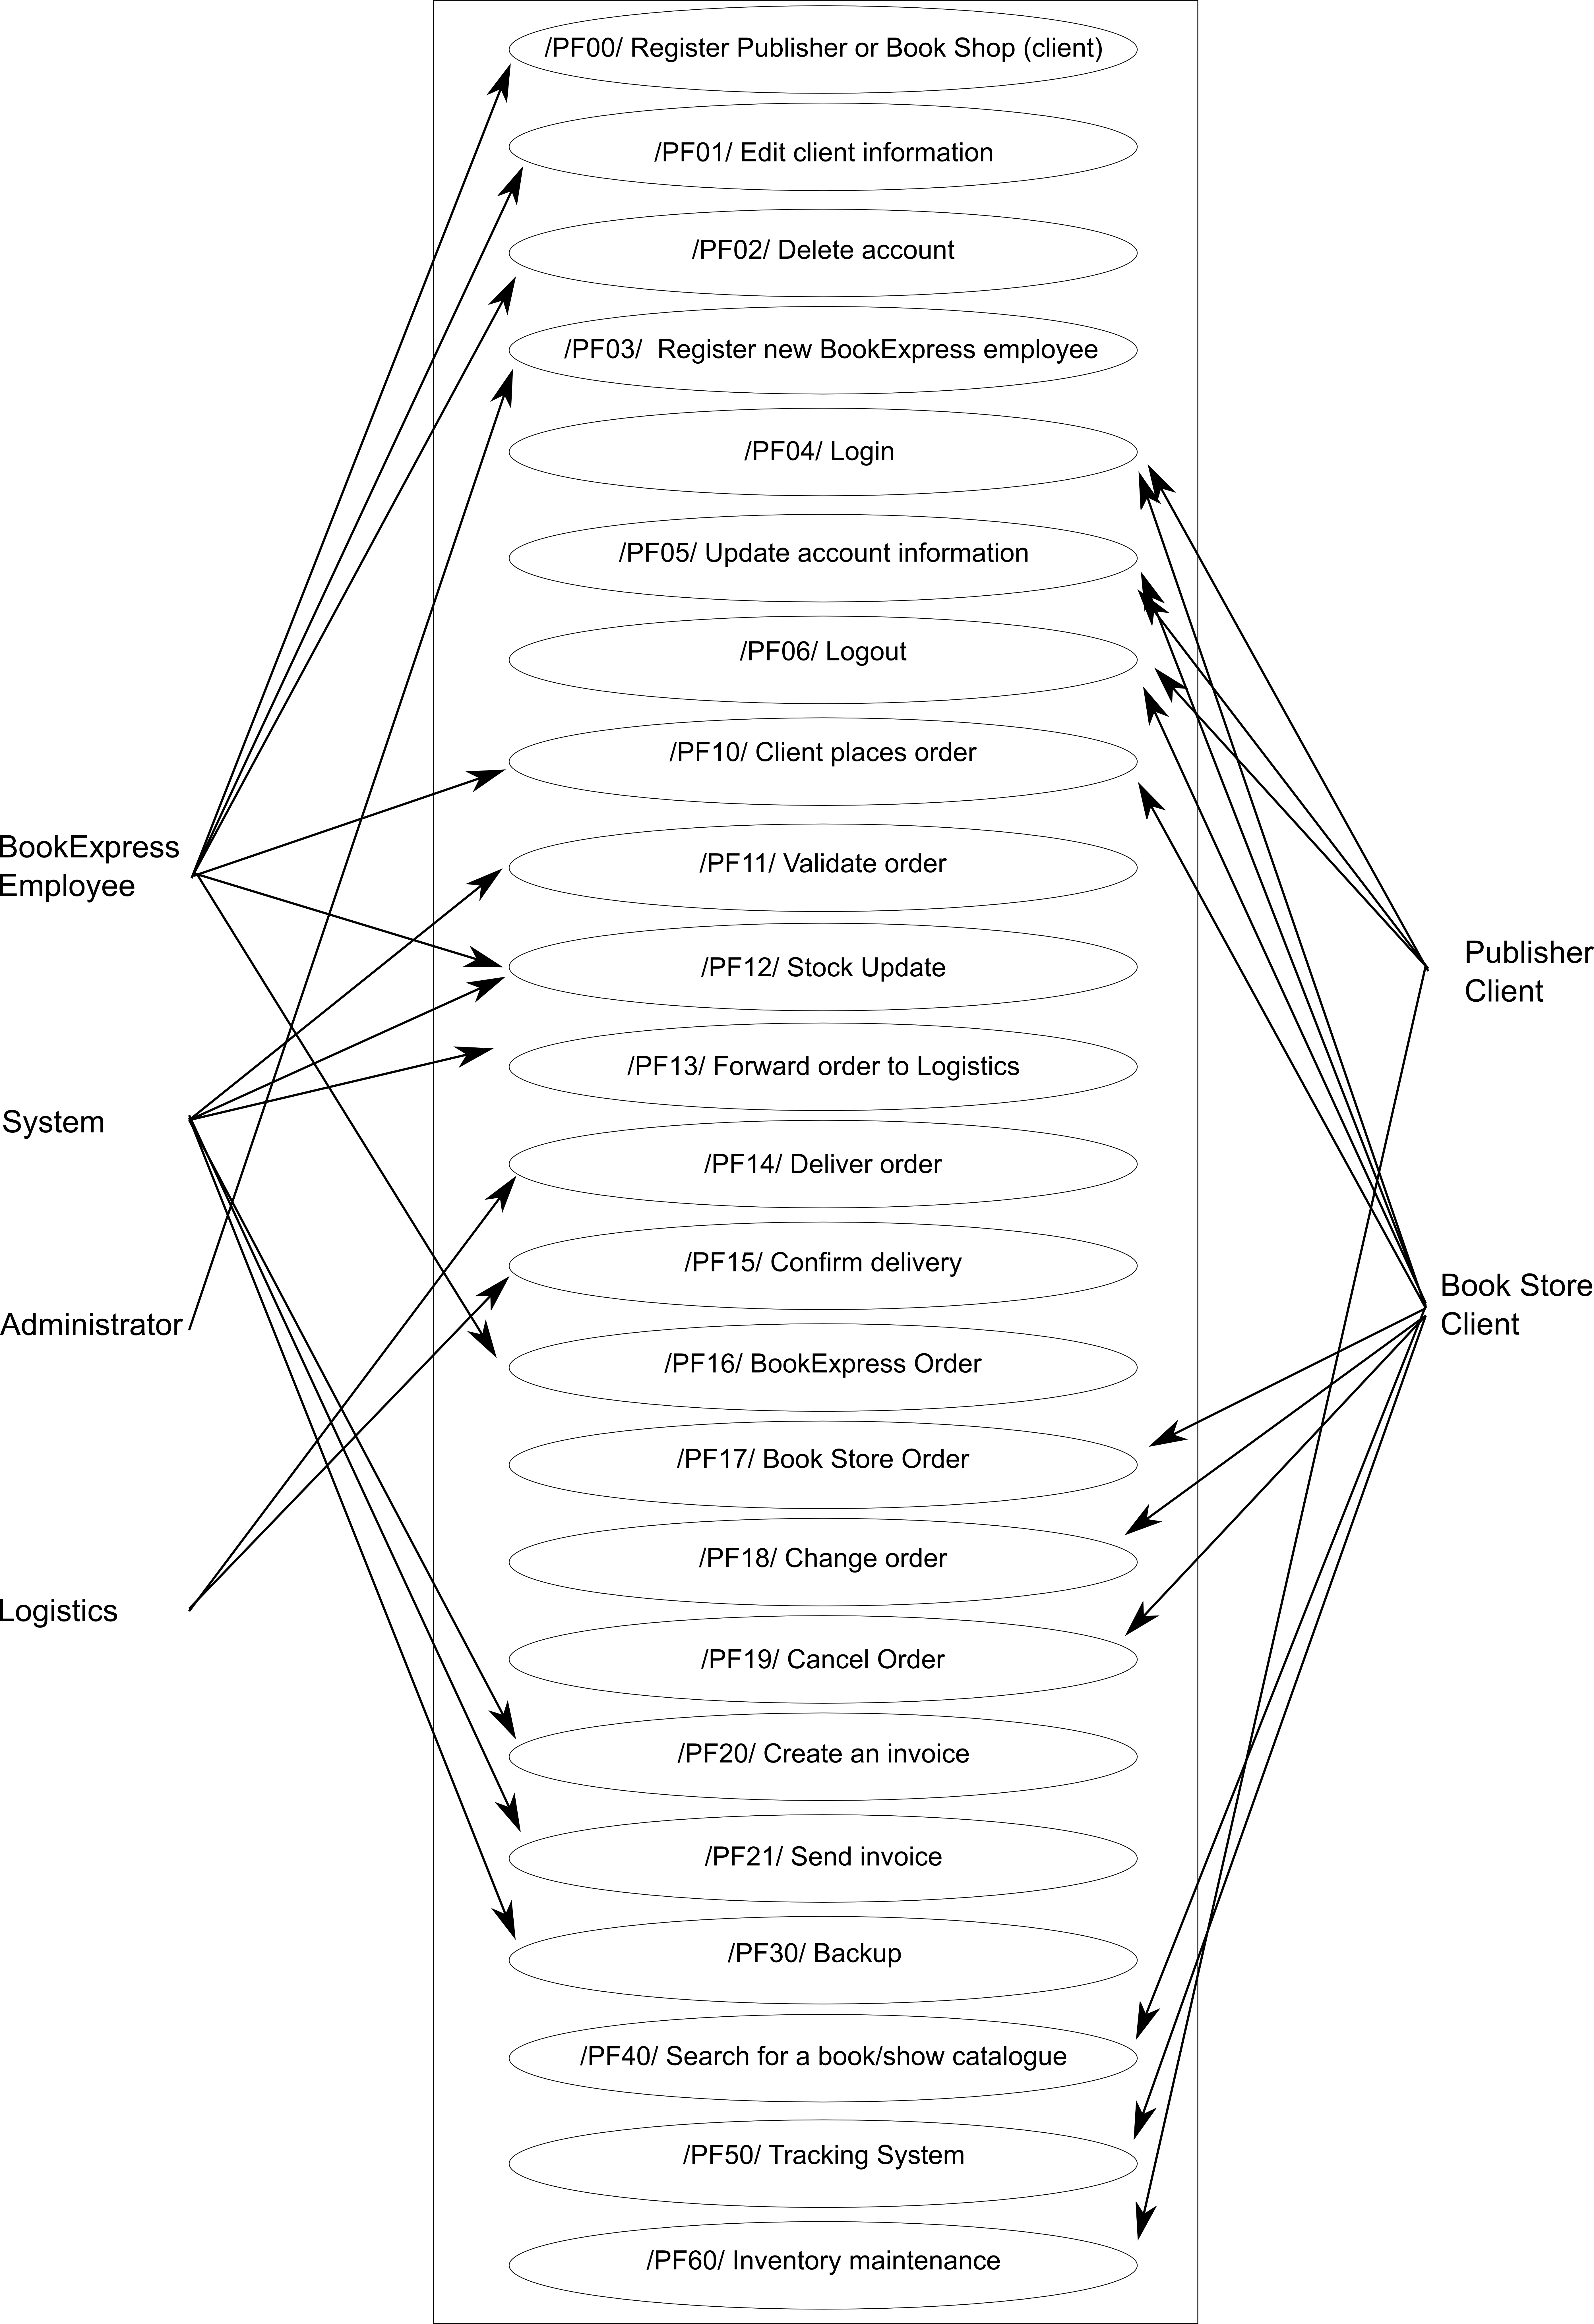
\includegraphics[width=\textwidth]{diagrams/BusinessProcessDiagram.png}
 \end{center}
 \caption{The environmental view of the product}
\end{figure}

\chapter{Product Functions}
\label{sec:product-functions}

\section{Internal}
\subsection{Employees of ``BookExpress''}

\begin{table}[H]
\centering
\begin{tabular}{p{1.5cm}p{3cm}p{8cm}}
\cellcolor{white}/PF00/	& \textbf{Process}	& Register Publisher or Book Shop (client)\\
\cellcolor{white}		& \textbf{Actor(s)} & BookExpress employee\\
\cellcolor{white}		& \textbf{Category} & Must have\\
\cellcolor{white}		& \textbf{Description}	 & A Book Express employee creates an account for a book shop or publisher after both business partners have signed a contract handling the business relations.\\
\cellcolor{white}		& \textbf{Goal} & The contract partner should have an account to log into the Software. After registration through the Book Express employee, the contract partner will be send a verification and its information via email.\\
\cellcolor{white}		& \textbf{Preconditions} & Contract signed\\
\cellcolor{white}		& \textbf{Postcondition success} & Successfully created account\\
\cellcolor{white}		& \textbf{Postcondition failure} & Unsuccessful in creating an account\\
\cellcolor{white}		& \textbf{Trigger} & Menu option "register new client" (Software)\\
\cellcolor{white}		& \textbf{Sequence} & Input relevant data and contractor details into the managements system\\
\cellcolor{white}		& & Save the signed contract on the server\\
\cellcolor{white}		& & Register a new client by creating a new PIN in the database\\
\cellcolor{white}		& & Send verification and account information to the contractor\\
\cellcolor{white}\hfill \\		
\end{tabular}
\caption{/PF00/ Register Publisher or Book Shop}
\label{tab:pf00}
\end{table}

\begin{table}[H]
\centering
\begin{tabular}{p{1.5cm}p{3cm}p{8cm}}
\cellcolor{white}/PF01/	& \textbf{Process} & Edit client information\\
\cellcolor{white}		& \textbf{Actor(s)} & BookExpress employee\\
\cellcolor{white}		& \textbf{Category} & Must have\\
\cellcolor{white}		& \textbf{Description}	 & The clients data is outdated and needs to be updated\\
\cellcolor{white}		& \textbf{Goal} & Client data is updated\\
\cellcolor{white}		& \textbf{Preconditions} & Client exists in database\\
\cellcolor{white}		& \textbf{Postcondition success} & Client data is updated and a notification mail is sent to the client.\\
\cellcolor{white}		& \textbf{Postcondition failure} & Client data is not updated but rolled back to the previous state. Notification with problem report is shown to the employee.\\
\cellcolor{white}		& \textbf{Trigger} & Menu option "edit client data" (Software)\\
\cellcolor{white}		& \textbf{Sequence} & Menu option "edit client data"\\
\cellcolor{white}		& & Edit specific data\\
\cellcolor{white}		& & Submit edited data to the server\\
\cellcolor{white}\hfill \\
\end{tabular}
\caption{/PF01/ Edit client information}
\label{tab:pf01}
\end{table}

\begin{table}[H]
\centering
\begin{tabular}{p{1.5cm}p{3cm}p{8cm}}
\cellcolor{white}/PF02/	& \textbf{Process} & Delete account\\ 
\cellcolor{white}		& \textbf{Actor(s)} & BookExpress Employee\\ 
\cellcolor{white}		& \textbf{Category} & Must have\\
\cellcolor{white}		& \textbf{Description}	 & Client gets deleted due to resignation of the contract\\ 
\cellcolor{white}		& \textbf{Goal} & Delete client from the system\\
\cellcolor{white}		& \textbf{Preconditions} & Client exists in database\\
\cellcolor{white}		& & Contract is being resigned by one of the contractors\\
\cellcolor{white}		& \textbf{Postcondition success} & Client is deleted from the system\\
\cellcolor{white}		& \textbf{Postcondition failure} & Client could not be deleted because of existing orders\\
\cellcolor{white}		& \textbf{Trigger} & Menu option "delete client" (Software)\\
\cellcolor{white}		& \textbf{Sequence} & Choose client\\
\cellcolor{white}		& & Check if client is deletable (i.e. no existing orders)\\
\cellcolor{white}		& & Send notification mail to client\\
\cellcolor{white}		& & Delete client\\
\cellcolor{white}\hfill \\		
\end{tabular}
\caption{/PF02/ Delete Account}
\label{tab:pf02}
\end{table}


\begin{table}[H]
\centering
\begin{tabular}{p{1.5cm}p{3cm}p{8cm}}
\cellcolor{white}	 /PF10/	& \textbf{Process} & Client places order via Phone\\ 
\cellcolor{white}		& \textbf{Category} & Must have\\
\cellcolor{white}		& \textbf{Actor(s)} & BookExpress employee, client\\ 
\cellcolor{white}		& \textbf{Description}	 & A client orders book via telephone\\ 
\cellcolor{white}		& \textbf{Goal} & Order is placed in an order queue\\
\cellcolor{white}		& \textbf{Preconditions} & Client exists in database\\
\cellcolor{white}		& & Client is authorized\\
\cellcolor{white}		& \textbf{Postcondition success} & Order status is set to "Processing"\\
\cellcolor{white}		& \textbf{Postcondition failure} & -\\
\cellcolor{white}		& \textbf{Trigger} & Client initiates order process by calling a BookExpress employee\\
\cellcolor{white}		& & BookExpress employee triggers manual order process\\
\cellcolor{white}		& \textbf{Sequence} & BookExpress employee selects client in Software\\
\cellcolor{white}		& & BookExpress employee enters ordered book into the system\\
\cellcolor{white}		& & Set order status to "Processing"\\
\cellcolor{white}		& & Order notification containing detailed report is sent to client\\
\cellcolor{white}\hfill \\
\end{tabular}
\caption{/PF10/ Client places order via Phone}
\label{tab:pf10}
\end{table}

\begin{table}[H]
\centering
\begin{tabular}{p{1.5cm}p{3cm}p{8cm}}
\cellcolor{white}	 /PF11/	& \textbf{Process} & Validate order\\ 
\cellcolor{white}		& \textbf{Category} & Must have\\
\cellcolor{white}		& \textbf{Actor(s)} & System\\ 
\cellcolor{white}		& \textbf{Description}	 & Order is checked as valid\\ 
\cellcolor{white}		& \textbf{Goal} & The software checks every order for validation and confirms it to the client. BookExpress knows about every orders validation status.\\
\cellcolor{white}		& \textbf{Preconditions} & Order status is "Processing"\\
\cellcolor{white}		& \textbf{Postcondition success} & Client receives a confirmation email and order status is set to "Valid"\\
\cellcolor{white}		& \textbf{Postcondition failure} & Client receives a problem report about invalid order and status is set to "Invalid"\\
\cellcolor{white}		& \textbf{Trigger} & Order was placed and status is set to "Processing"\\
\cellcolor{white}		& \textbf{Sequence} & System  gathers details and checks whether order is valid or not\\
\cellcolor{white}		& & System sends mail to client\\
\cellcolor{white}\hfill \\
\end{tabular}
\caption{/PF11/ Validate Order}
\label{tab:pf11}
\end{table}

\begin{table}[H]
\centering
\begin{tabular}{p{1.5cm}p{3cm}p{8cm}}
\cellcolor{white}	 /PF12/	& \textbf{Process} & Stock Update\\ 
\cellcolor{white}		& \textbf{Category} & Must have\\
\cellcolor{white}		& \textbf{Actor(s)} & System/BookExpress employee\\ 
\cellcolor{white}		& \textbf{Description}	 & The employee in charge of the stock checks the availability of all books and updates the stock accordingly.\\ 
\cellcolor{white}		& \textbf{Goal} & Check succeeds\\
\cellcolor{white}		& \textbf{Preconditions} & Order is placed or BookExpress employee initiates check\\
\cellcolor{white}		& \textbf{Postcondition success} & Books which are nearly out of stock get displayed as a list\\
\cellcolor{white}		& \textbf{Postcondition failure} & -\\
\cellcolor{white}		& \textbf{Trigger} & Stock check is initiated\\
\cellcolor{white}		& \textbf{Sequence} & Check if a book is available in an sufficient amount\\
\cellcolor{white}		& & Make a list of all books which need to be ordered\\
\cellcolor{white}		& & Submit list to system\\
\cellcolor{white}\hfill \\
\end{tabular}
\caption{/PF12/ Stock Update}
\label{tab:pf12}
\end{table}

\begin{table}[H]
\centering
\begin{tabular}{p{1.5cm}p{3cm}p{8cm}}
\cellcolor{white}	 /PF13/	& \textbf{Process} & Forward order to Logistics\\ 
\cellcolor{white}		& \textbf{Category} & Primary\\
\cellcolor{white}		& \textbf{Actor(s)} & System\\ 
\cellcolor{white}		& \textbf{Description}	 & A validated order gets forwarded to Logistics\\ 
\cellcolor{white}		& \textbf{Goal} & Logistics proceeds processing the order\\
\cellcolor{white}		& \textbf{Preconditions} & Order is valid\\
\cellcolor{white}		& \textbf{Postcondition success} & Logistics processes delivery and order satus is set to "Logistics"\\
\cellcolor{white}		& \textbf{Postcondition failure} & Order could not be forwarded to Logistics\\
\cellcolor{white}		& \textbf{Trigger} & Order status is set to "Valid"\\
\cellcolor{white}		& \textbf{Sequence} & Send order information/details to Logistics and set order status to "Logistics"\\
\cellcolor{white}\hfill \\
\end{tabular}
\caption{/PF13/ Forward order to Logistics}
\label{tab:pf13}
\end{table}

\begin{table}[H]
\centering
\begin{tabular}{p{1.5cm}p{3cm}p{8cm}}
\cellcolor{white}/PF14/	& \textbf{Process} & Deliver order\\
\cellcolor{white}		& \textbf{Actor(s)} & System\\
\cellcolor{white}		& \textbf{Category} & Primary\\
\cellcolor{white}		& \textbf{Description}	 &  The order is send to the book store\\
\cellcolor{white}		& \textbf{Goal} & Deliver ordered books\\
\cellcolor{white}		& \textbf{Preconditions} & Order status is "Logistics"\\
\cellcolor{white}		& & Books are available in stock\\
\cellcolor{white}		& \textbf{Postcondition success} & Order status is set to "Delivery"\\
\cellcolor{white}		& \textbf{Postcondition failure} & Order could not be marked as "Delivery"\\
\cellcolor{white}		& \textbf{Trigger} & Forward order to Logistics\\
\cellcolor{white}		& \textbf{Sequence} & Check if books are in stock\\
\cellcolor{white}		& & Receive book store information\\
\cellcolor{white}		& & Deliver order to book store\\
\cellcolor{white}		& & Set order status to "Delivery"\\
\cellcolor{white}\hfill \\
\end{tabular}
\caption{/PF14/ Deliver Order}
\label{tab:pf14}
\end{table}


\begin{table}[H]
\centering
\begin{tabular}{p{1.5cm}p{3cm}p{8cm}}
\cellcolor{white}/PF15/	& \textbf{Process} & Confirm delivery\\
\cellcolor{white}		& \textbf{Actor(s)} & Employee (Logistics)\\
\cellcolor{white}		& \textbf{Category} & Primary\\
\cellcolor{white}		& \textbf{Description}	 & Logistics confirms the correct delivery of an order\\
\cellcolor{white}		& \textbf{Goal} & Delivery is successful\\
\cellcolor{white}		& \textbf{Preconditions} & Order is marked as sent\\
\cellcolor{white}		& \textbf{Postcondition success} & Order status is set to "Delivered"\\
\cellcolor{white}		& \textbf{Postcondition failure} & Order could not be set to "Delivered"\\
\cellcolor{white}		& \textbf{Trigger} & Deliver order\\
\cellcolor{white}		& \textbf{Sequence} & Get delivery status\\
\cellcolor{white}		& & Order status is set to "Delivered"\\
\cellcolor{white}\hfill \\
\end{tabular}
\caption{/PF15/ Confirm Delivery}
\label{tab:pf15}
\end{table}

\begin{table}[H]
\centering
\begin{tabular}{p{1.5cm}p{3cm}p{8cm}}
\cellcolor{white}/PF16/	& \textbf{Process} & BookExpress Order\\
\cellcolor{white}		& \textbf{Actor(s)} & BookExpress employee\\
\cellcolor{white}		& \textbf{Category} & Must have\\
\cellcolor{white}		& \textbf{Description}	 & The Employee orders a number of books from the publisher\\
\cellcolor{white}		& \textbf{Goal} & Order books from a publisher\\
\cellcolor{white}		& \textbf{Preconditions} & need for new books\\
\cellcolor{white}		& \textbf{Postcondition success} & Books are ordered and publisher gets an notification mail\\
\cellcolor{white}		& \textbf{Postcondition failure} & -\\
\cellcolor{white}		& \textbf{Trigger} & BookExpress employee initates an order\\
\cellcolor{white}		& \textbf{Sequence} & Select books from list or search\\
\cellcolor{white}		& & Submit list to publisher\\
\cellcolor{white}\hfill \\
\end{tabular}
\caption{/PF16/ BookExpress Order}
\label{tab:pf16}
\end{table}

\begin{table}[H]
\centering
\begin{tabular}{p{1.5cm}p{3cm}p{8cm}}
\cellcolor{white}/PF20/	& \textbf{Process} & Create an invoice\\
\cellcolor{white}		& \textbf{Actor(s)} & System\\
\cellcolor{white}		& \textbf{Category} & Secondary\\
\cellcolor{white}		& \textbf{Description}	 & The system creates an invoice \\
\cellcolor{white}		& \textbf{Goal} & Documenting order and deliver it with invoice\\
\cellcolor{white}		& \textbf{Preconditions} & Order is valid\\
\cellcolor{white}		& \textbf{Postcondition success} & Invoice successfully created\\
\cellcolor{white}		& \textbf{Postcondition failure} & Invoice could not be created\\
\cellcolor{white}		& & Check information about order\\
\cellcolor{white}		& \textbf{Trigger} & Order status is "Valid"\\
\cellcolor{white}		& \textbf{Sequence} & Create an entry in database\\
\cellcolor{white}		& & List the ordered books with price\\
\cellcolor{white}		& & List tax to invoice\\
\cellcolor{white}\hfill \\
\end{tabular}
\caption{/PF20/ Create an invoice}
\label{tab:pf20}
\end{table}

\begin{table}[H]
\centering
\begin{tabular}{p{1.5cm}p{3cm}p{8cm}}
\cellcolor{white}/PF21/	& \textbf{Process} & Send invoice\\
\cellcolor{white}		& \textbf{Actor(s)} & System\\
\cellcolor{white}		& \textbf{Category} & Secondary\\
\cellcolor{white}		& \textbf{Description}	 & The invoice is send to the book store via mail\\
\cellcolor{white}		& \textbf{Goal} & Inform the book shop\\
\cellcolor{white}		& \textbf{Preconditions} & Successful created invoice\\
\cellcolor{white}		& \textbf{Postcondition success} & Book store receives a notification mail\\
\cellcolor{white}		& \textbf{Postcondition failure} & -\\
\cellcolor{white}		& \textbf{Trigger} & Creation of an invoice\\
\cellcolor{white}		& \textbf{Sequence} & Get invoice\\
\cellcolor{white}		& & Send invoice to book store\\
\cellcolor{white}\hfill \\
\end{tabular}
\caption{/PF21/ Send invoice}
\label{tab:pf21}
\end{table}

\begin{table}[H]
\centering
\begin{tabular}{p{1.5cm}p{3cm}p{8cm}}
\cellcolor{white}/PF30/	& \textbf{Process} & Backup\\
\cellcolor{white}		& \textbf{Actor(s)} & System\\
\cellcolor{white}		& \textbf{Category} & Primary\\
\cellcolor{white}		& \textbf{Description}	 & A backup of the complete databases must be done. This should happen periodically and save all data on a server.\\
\cellcolor{white}		& \textbf{Goal} & In case of a crash, every data must be saves as a preventative backup\\
\cellcolor{white}		& \textbf{Preconditions} & Server for the backup\\
\cellcolor{white}		& \textbf{Postcondition success} & Successful backup in periodical intervals\\
\cellcolor{white}		& \textbf{Postcondition failure} & A notification will be send to the administrator of the system\\
\cellcolor{white}		& \textbf{Trigger} & Configured time to start a backup\\
\cellcolor{white}		& \textbf{Sequence} & Start Backup\\
\cellcolor{white}		& & Place backup on the backup server\\
\cellcolor{white}\hfill \\
\end{tabular}
\caption{/PF30/ Backup}
\label{tab:pf30}
\end{table}


\section{External}

\subsection{Book Stores and Publishers}

\begin{table}[H]
\centering
\begin{tabular}{p{1.5cm}p{3cm}p{8cm}}
\cellcolor{white}/PF03/	& \textbf{Process} & Login\\
\cellcolor{white}		& \textbf{Actor(s)} & Book store/publisher\\
\cellcolor{white}		& \textbf{Category} & Must have\\
\cellcolor{white}		& \textbf{Description}	 & The user logs on with his PIN and password\\
\cellcolor{white}		& \textbf{Goal} & Provide a fully functional system to the user\\
\cellcolor{white}		& \textbf{Preconditions} & Existing account\\
\cellcolor{white}		& \textbf{Postcondition success} & Successful login\\
\cellcolor{white}		& \textbf{Postcondition failure} & Unsuccessful login caused by a wrong PIN or password\\
\cellcolor{white}		& \textbf{Trigger} & Menu Option "Login"\\
\cellcolor{white}		& \textbf{Sequence} & Enter PIN\\
\cellcolor{white}		& & Enter password\\
\cellcolor{white}		& & Validity of data is checked by the System\\
\cellcolor{white}		& & Login successful or display an error message in case of unsuccessful login\\
\cellcolor{white}\hfill \\
\end{tabular}
\caption{/PF03/ Login}
\label{tab:pf03}
\end{table}

\begin{table}[H]
\centering
\begin{tabular}{p{1.5cm}p{3cm}p{8cm}}
\cellcolor{white}/PF04/	& \textbf{Process} & Update account information\\
\cellcolor{white}		& \textbf{Actor(s)} & Book store/publisher\\
\cellcolor{white}		& \textbf{Category} & Must have\\
\cellcolor{white}		& \textbf{Description}	 & The user is able to edit/update its account information (e.g. address, correspondent etc.)\\
\cellcolor{white}		& \textbf{Goal} & User is able to update changes\\
\cellcolor{white}		& \textbf{Preconditions} & User is logged on\\
\cellcolor{white}		& \textbf{Postcondition success} & Updating the account succeeded\\
\cellcolor{white}		& \textbf{Postcondition failure} & Updating the account failed\\
\cellcolor{white}		& \textbf{Trigger} & Menu option "edit\\
\cellcolor{white}		& \textbf{Sequence} & Edit specific data\\
\cellcolor{white}		& & System checks correctness of data (e.g. email format etc.)\\
\cellcolor{white}		& & Submit edited data to the server\\
\cellcolor{white}\hfill \\
\end{tabular}
\caption{/PF04/ Update account information}
\label{tab:pf04}
\end{table}

\begin{table}[H]
\centering
\begin{tabular}{p{1.5cm}p{3cm}p{8cm}}
\cellcolor{white}/PF05/	& \textbf{Process} & Logout\\
\cellcolor{white}		& \textbf{Actor(s)} & Book store/publisher\\
\cellcolor{white}		& \textbf{Category} & Must have\\
\cellcolor{white}		& \textbf{Description}	 & User logs out\\
\cellcolor{white}		& \textbf{Goal} & User is logged out\\
\cellcolor{white}		& \textbf{Preconditions} & User is logged in\\
\cellcolor{white}		& \textbf{Postcondition success} & Successful logout\\
\cellcolor{white}		& \textbf{Postcondition failure} & Unsuccessful logout caused by an abort of the user\\
\cellcolor{white}		& \textbf{Trigger} & Menu option "Logout"\\
\cellcolor{white}		& \textbf{Sequence} & User confirms to log out\\
\cellcolor{white}		& & The system terminates the current session\\
\cellcolor{white}\hfill \\
\end{tabular}
\caption{/PF05/ Logout}
\label{tab:pf05}
\end{table}


\subsection{Book Stores (``Clients'')}

\begin{table}[H]
\centering
\begin{tabular}{p{1.5cm}p{3cm}p{8cm}}
\cellcolor{white}	 /PF40/	& \textbf{Process} & Search for a book/show catalogue\\ 
\cellcolor{white}		& \textbf{Category} & Must have\\
\cellcolor{white}		& \textbf{Actor(s)} & Client\\ 
\cellcolor{white}		& \textbf{Description}	 & Client searches for a book to add it to his order\\ 
\cellcolor{white}		& \textbf{Goal} & Searching for a book succeeded\\
\cellcolor{white}		& \textbf{Preconditions} & Client is logged into the system\\
\cellcolor{white}		& \textbf{Postcondition success} & Book is being found\\
\cellcolor{white}		& & Display items and options\\
\cellcolor{white}		& \textbf{Postcondition failure} & Book could not be found\\
\cellcolor{white}		& & Display notification\\
\cellcolor{white}		& \textbf{Trigger} & Menu option "find books" (Software)\\
\cellcolor{white}		& \textbf{Sequence} & Enter ISBN/title/author/genre in search bar\\
\cellcolor{white}		& & Hit the "Search"-Button\\
\cellcolor{white}		& & Choose book from list to add it to the order\\
\cellcolor{white}\hfill \\
\end{tabular}
\caption{/PF40/ Search for a book/show catalogue}
\label{tab:pf40}
\end{table}

\begin{table}[H]
\centering
\begin{tabular}{p{1.5cm}p{3cm}p{8cm}}
\cellcolor{white}/PF17/	& \textbf{Process} & Book Store Order\\ 
\cellcolor{white}		& \textbf{Category} & Must have\\
\cellcolor{white}		& \textbf{Actor(s)} & Book Store Employee\\ 
\cellcolor{white}		& \textbf{Description}	 & The Book Store orders a book from BookExpress.
This can either happen through a constant connection where every order is individually processed or the store can choose to collect orders internally and send them
as one big order.\\ 
\cellcolor{white}		& \textbf{Goal} & Order is placed\\
\cellcolor{white}		& \textbf{Preconditions} & Client is successfully logged into the web interface\\
\cellcolor{white}		& & Connection to BookExpress server is established\\
\cellcolor{white}		& \textbf{Postcondition success} & Order is delivered to BookExpress  and the order status is set to "Processing"\\
\cellcolor{white}		& \textbf{Postcondition failure} & Order is saved as draft and client gets a notification\\
\cellcolor{white}		& \textbf{Trigger} & Menu Option "create new order" (Web interface)\\
\cellcolor{white}		& \textbf{Sequence} & Client adds books to order (via book search or ISBN)\\
\cellcolor{white}		& & Client specifies amount for every book\\
\cellcolor{white}		& & Client submits order to server\\
\cellcolor{white}		& & Order status is set to "Processing"\\
\cellcolor{white}\hfill \\
\end{tabular}
\caption{/PF17/ Book Store Order}
\label{tab:pf17}
\end{table}

\begin{table}[H]
\centering
\begin{tabular}{p{1.5cm}p{3cm}p{8cm}}
\cellcolor{white}/PF18/	& \textbf{Process} & Change order\\
\cellcolor{white}		& \textbf{Actor(s)} & Book store\\
\cellcolor{white}		& \textbf{Category} & Must have\\
\cellcolor{white}		& \textbf{Description}	 & As long as the order is not validated, the user can change information\\
\cellcolor{white}		& \textbf{Goal} & User can correct an order\\
\cellcolor{white}		& \textbf{Preconditions} & Order exists and user is logged in. Order status is set to "Processing"\\
\cellcolor{white}		& \textbf{Postcondition success} & Order information successfully changed\\
\cellcolor{white}		& \textbf{Postcondition failure} & Order information could not be changed because the order is already being validated\\
\cellcolor{white}		& \textbf{Trigger} & Menu option "Change order"\\
\cellcolor{white}		& \textbf{Sequence} & Select order to be changed\\
\cellcolor{white}		& & System checks validity status of the order\\
\cellcolor{white}		& & If not validated, user can change order information\\
\cellcolor{white}		& & Submit changes to the System\\
\cellcolor{white}		& & User receives a confirmation mail\\
\cellcolor{white}\hfill \\
\end{tabular}
\caption{/PF18/ Change order}
\label{tab:pf18}
\end{table}

\begin{table}[H]
\centering
\begin{tabular}{p{1.5cm}p{3cm}p{8cm}}
\cellcolor{white}/PF19/	& \textbf{Process} & Cancel Order\\
\cellcolor{white}		& \textbf{Actor(s)} & Book Store Employee\\
\cellcolor{white}		& \textbf{Category} & Must have\\
\cellcolor{white}		& \textbf{Description}	 & The employee at the book store can cancel the order if the status isn't already set to "Delivery"\\
\cellcolor{white}		& \textbf{Goal} & Current orders can be cancelled\\
\cellcolor{white}		& \textbf{Preconditions} & Order exists\\
\cellcolor{white}		& \textbf{Postcondition success} & Order successfully cancelled. Book Store receives a confirmation mail\\
\cellcolor{white}		& \textbf{Postcondition failure} & Book Store receives a problem report\\
\cellcolor{white}		& \textbf{Trigger} & Menu option "cancel order"\\
\cellcolor{white}		& \textbf{Sequence} & Select order to cancel\\
\cellcolor{white}		& & Check whether order status isn't set to "Delivery" or "Delivered"\\
\cellcolor{white}		& & Set order status to "Canceled"\\
\cellcolor{white}\hfill \\
\end{tabular}
\caption{/PF19/ Cancel Order}
\label{tab:pf19}
\end{table}

\begin{table}[H]
\centering
\begin{tabular}{p{1.5cm}p{3cm}p{8cm}}
\cellcolor{white}/PF50/	& \textbf{Process} & Tracking System\\
\cellcolor{white}		& \textbf{Actor(s)} & Book Store Employee\\
\cellcolor{white}		& \textbf{Category} & Must have\\
\cellcolor{white}		& \textbf{Description}	 & Every Client, Publisher or BookExpress employee can look up at which stage the order is right now, e.g. processing or shipping to BookExpress/the book store.\\
\cellcolor{white}		& \textbf{Goal} & Look up order information/status\\
\cellcolor{white}		& \textbf{Preconditions} & Order exists\\
\cellcolor{white}		& \textbf{Postcondition success} & Employee receives information/status of order\\
\cellcolor{white}		& \textbf{Postcondition failure} & -\\
\cellcolor{white}		& \textbf{Trigger} & Menu option "tracking system"\\
\cellcolor{white}		& \textbf{Sequence} & Select order to track\\
\cellcolor{white}\hfill \\
\end{tabular}
\caption{/PF50/ Tracking System}
\label{tab:pf50}
\end{table}


\subsection{Publishers}

\begin{table}[H]
\centering
\begin{tabular}{p{1.5cm}p{3cm}p{8cm}}
\cellcolor{white}/PF60/	& \textbf{Process} & Inventory maintenance\\
\cellcolor{white}		& \textbf{Actor(s)} & Publisher\\
\cellcolor{white}		& \textbf{Category} & Must have\\
\cellcolor{white}		& \textbf{Description}	 & Publishers can update their inventory list
(i.e. the list of available books) either via mail or using the direct connection over the web-based interface.\\
\cellcolor{white}		& \textbf{Goal} & Updated inventory list\\
\cellcolor{white}		& \textbf{Preconditions} & Publisher exists\\
\cellcolor{white}		& \textbf{Postcondition success} & Send success mail to publisher\\
\cellcolor{white}		& \textbf{Postcondition failure} & Send problem report to publisher\\
\cellcolor{white}		& \textbf{Trigger} & Menu option "inventory maintenance" (Software) or via mail\\
\cellcolor{white}		& \textbf{Sequence} & Edit inventory list\\
\cellcolor{white}		& & Submit list to server\\
\cellcolor{white}\hfill \\
\end{tabular}
\caption{/PF60/ Inventory maintenance}
\label{tab:pf60}
\end{table}


\chapter{Product Data}
\section{User Data}
\subsection{Book Stores}

\rowcolors{1}{tableEven}{tableOdd}

\begin{table}[H]
\centering
\begin{tabular}{llp{8.75cm}}
\cellcolor{white}/PD20/	& \textbf{Data}			& Book Store Data\\
\cellcolor{white}		& \textbf{Composition}	& Name, PIN, Address, Correspondent, E-Mail Address, Phone Number, Contract Data\\
\cellcolor{white}		& \textbf{Size}		& approx 10,000\\
\cellcolor{white}		& \textbf{Traffic}		& Low\\
\end{tabular} 
\caption{/PD20/ Book Store Data}
\label{tab:pd20}
\end{table}

\subsection{Publishers}
\begin{table}[H]
\centering
\begin{tabular}{llp{8.75cm}}
\cellcolor{white}/PD30/	& \textbf{Data}			& Publisher Data\\
\cellcolor{white}		& \textbf{Composition}	& Name, PIN, Address, Correspondent, E-Mail Address, Phone Number, Contract Data\\
\cellcolor{white}		& \textbf{Size}		& approx 15,000\\
\cellcolor{white}		& \textbf{Traffic}		& Low\\
\end{tabular}
\caption{/PD30/ Publisher Data}
\label{tab:pd30}
\end{table}


\section{Order Data}
\begin{table}[H]
\centering
\begin{tabular}{llp{8.75cm}}
\cellcolor{white}/PD40/	& \textbf{Data}			& Order Data\\
\cellcolor{white}		& \textbf{Composition}	& PIN, ISBN, Amount, Price, Date, Current Ordering State\\
\cellcolor{white}		& \textbf{Size}		& 500,000\\
\cellcolor{white}		& \textbf{Traffic}		& Very High\\
\cellcolor{white}\hfill \\
\cellcolor{white}/PD41/	& \textbf{Data}			& Order Data History\\
\cellcolor{white}		& \textbf{Composition}	& PIN, ISBN, Amount, Price, Date\\
\cellcolor{white}		& \textbf{Size}		& 2,500,000\\
\cellcolor{white}		& \textbf{Traffic}		& High\\
\cellcolor{white}\hfill \\
\cellcolor{white}/PD42/	& \textbf{Data}			& Invoice Data\\
\cellcolor{white}		& \textbf{Composition}	& Order Data, Book Store Data, PIN, Invoice Status\\
\cellcolor{white}		& \textbf{Size}		& 500,000\\
\cellcolor{white}		& \textbf{Traffic}		& Very High\\
\end{tabular}
\caption{/PD40/ Order Data, /PD41/ Order Data History, /PD42/ Invoice Data}
\label{tab:pd40+}
\end{table}


\section{Internal Data}
\subsection{Book Stock}
\begin{table}[H]
\centering
\begin{tabular}{llp{8.75cm}}
\cellcolor{white}/PD10/	& \textbf{Data}			& Book Data\\
\cellcolor{white}		& \textbf{Composition}	& ISBN, UPC/EAN, Title, Author, Publisher, Availability\\
\cellcolor{white}		& \textbf{Size}		& approx 1,500,000\\
\cellcolor{white}		& \textbf{Traffic}		& Average\\
\cellcolor{white}\hfill \\
\cellcolor{white}/PD11/	& \textbf{Data}			& Stock Data\\
\cellcolor{white}		& \textbf{Composition}	& Book Data, Availability\\
\cellcolor{white}		& \textbf{Size}		& approx 1,500,000\\
\cellcolor{white}		& \textbf{Traffic}		& Average\\
\end{tabular}
\caption{/PD10/ Book Data, /PD11/ Stock Data}
\label{tab:pd10+}
\end{table}

\subsection{Truck Information}
\begin{table}[H]
\centering
\begin{tabular}{llp{8.75cm}}
\cellcolor{white}/PD50/	& \textbf{Data}			& Truck Fleet Data\\
\cellcolor{white}		& \textbf{Composition}	& Driver, Registration Number, Truck Status\\
\cellcolor{white}		& \textbf{Size}		& 1,000\\
\cellcolor{white}		& \textbf{Traffic}		& Average\\
\end{tabular}
\caption{/PD50/ Truck Fleet Data}
\label{tab:pd50}
\end{table}

\subsection{Backup}
\begin{table}[H]
\centering
\begin{tabular}{llp{8.75cm}}
\cellcolor{white}/PD60/	& \textbf{Data}			& Backup\\
\cellcolor{white}		& \textbf{Composition}	& User Data, Order Data, Internal Data (except Backup)\\
\cellcolor{white}		& \textbf{Size}		& 5,000,000\\
\cellcolor{white}		& \textbf{Traffic}		& High\\
\end{tabular}
\caption{/PD60/ Backup}
\label{tab:pd60}
\end{table}

\chapter{Product Performance}
\section{System}
\begin{table}[H]
\centering
\begin{tabular}{llp{8.75cm}}
\cellcolor{white}/PP10/	& \textbf{Type}			& System (Web Interface)\\
\cellcolor{white}		& \textbf{Description}	& The Web Interface should be always reachable during business hours, but also 24/7 for quick changes. The availability outside business hours can be less than 100\% but should not fall below 99.7\%.\\
\cellcolor{white}		\hfill \\
\end{tabular}
\caption{/PP10/ System (Web Interface)}
\label{tab:pp10}
\end{table}

\begin{table}[H]
\centering
\begin{tabular}{llp{8.75cm}}
\cellcolor{white}/PP30/	& \textbf{Type}			& System (Order Processing)\\
\cellcolor{white}		& \textbf{Description}	& The order processing should always be reachable, confirming (or informing about, in case of error) any order.\\
\cellcolor{white}		\hfill \\
\end{tabular}
\caption{/PP30/ System (Order Processing)}
\label{tab:pp30}
\end{table}

\begin{table}[H]
\centering
\begin{tabular}{llp{8.75cm}}
\cellcolor{white}/PP40/	& \textbf{Type}			& System\\
\cellcolor{white}		& \textbf{Description}	& The System in general should be reliable and responsive all the time, taking not longer than 1-3 seconds for any request.\\
\cellcolor{white}		\hfill \\
\end{tabular}
\caption{/PP40/ System}
\label{tab:pp40}
\end{table}

\begin{table}[H]
\centering
\begin{tabular}{llp{8.75cm}}
\cellcolor{white}/PP50/	& \textbf{Type}			& System\\
\cellcolor{white}		& \textbf{Description}	& The response time criteria should also be met, when the processing limit of max. 2.000 simultaneous orders is reached.\\
\cellcolor{white}		\hfill \\
\end{tabular}
\caption{/PP50/ System}
\label{tab:pp50}
\end{table}

\section{Database}

\begin{table}[H]
\centering
\begin{tabular}{llp{8.75cm}}
\cellcolor{white}/PP20/	& \textbf{Type}			& Database (DB Connection)\\
\cellcolor{white}		& \textbf{Description}	& A Connection to the database should never be lost, an average uptime of 99.99\% has to be reached to satisfy any part of the system, currently needing data.\\
\cellcolor{white}		\hfill \\
\end{tabular}
\caption{/PP20/ Database (DB Connection)}
\label{tab:pp20}
\end{table}

\begin{table}[H]
\centering
\begin{tabular}{llp{8.75cm}}
\cellcolor{white}/PP21/	& \textbf{Type}			& Database (DB Backup)\\
\cellcolor{white}		& \textbf{Description}	& A database backup has to be initiated meeting the guidelines on general backup, also ensuring a consistent and complete history of any processed orders and any critical data.\\
\cellcolor{white}		\hfill \\
\end{tabular}
\caption{/PP21/ Database (DB Backup)}
\label{tab:pp21}
\end{table}

\section{Security}
\begin{table}[H]
\centering
\begin{tabular}{llp{8.75cm}}
\cellcolor{white}/PP60/	& \textbf{Type}			& Security (Stock Availability)\\
\cellcolor{white}		& \textbf{Description}	& Stock items should always be able to be ordered, ensuring fast delivery on order.\\
\cellcolor{white}		\hfill \\
\end{tabular}
\caption{/PP60/ Security (Stock Availability)}
\label{tab:pp60}
\end{table}

\begin{table}[H]
\centering
\begin{tabular}{llp{8.75cm}}
\cellcolor{white}/PP61/	& \textbf{Type}			& Security (Connection)\\
\cellcolor{white}		& \textbf{Description}	& Any connection issued to the system and between system components should be at least encrypted with 256 bit SSL.\\
\cellcolor{white}		\hfill \\
\end{tabular}
\caption{/PP61/ Security (Connection)}
\label{tab:pp61}
\end{table}

\begin{table}[H]
\centering
\begin{tabular}{llp{8.75cm}}
\cellcolor{white}/PP62/	& \textbf{Type}			& Security (Database)\\
\cellcolor{white}		& \textbf{Description}	& The database should be on an encrypted device, securing personal customer data.\\
\cellcolor{white}		\hfill \\
\end{tabular}
\caption{/PP62/ Security (Database)}
\label{tab:pp62}
\end{table}


\chapter{Quality Requirements}

\begin{center}

\rowcolors{1}{tableEven}{tableOdd}
\begin{table}[H]
\centering
\begin{tabular}{|lllll|}
\hline
\cellcolor{tableHead}Product Quality & \cellcolor{tableHead}excellent & \cellcolor{tableHead}good & \cellcolor{tableHead}normal & \cellcolor{tableHead}not applicable \\ 
\hline
Functionality &  &  &  &  \\ 
suitability &  & \checkmark &  &  \\ 
correctness & \checkmark &  &  &  \\ 
interoperability &  & \checkmark &  &  \\ 
conformity &  & \checkmark &  &  \\ 
security & \checkmark &  &  &  \\ 
Reliability &  &  &  &  \\ 
maturity &  & \checkmark &  &  \\ 
error tolerance &  & \checkmark &  &  \\ 
re-invoking & \checkmark &  &  &  \\ 
Usability &  &  &  &  \\ 
comprehensibility &  & \checkmark &  &  \\ 
learnability &  &  & \checkmark &  \\ 
ease of use &  & \checkmark &  &  \\ 
Efficiency &  &  &  &  \\ 
time behaviour & \checkmark &  &  &  \\ 
resource use &  &  & \checkmark &  \\ 
Maintainability &  &  &  &  \\ 
easy to analyse &  & \checkmark &  &  \\ 
easy to modify &  &  & \checkmark &  \\ 
stability & \checkmark &  &  &  \\ 
testability &  &  &  & \checkmark \\ 
Installability &  &  &  &  \\ 
adaptability &  &  & \checkmark &  \\ 
easy to install &  &  & \checkmark &  \\ 
conformity &  & \checkmark &  &  \\ 
exchangeability &  &  &  & \checkmark \\
\hline
\end{tabular}
\caption{Quality Requirements}
\label{tab:quality-requirements}
\end{table}

\end{center}

\chapter{User Interface}
Description of user interface elements for the client application and the web interface. Also a brief specification of the user rights management.

\section{Client Application (for clerks)}
\begin{table}[H]
\centering
\begin{tabular}{llp{8.75cm}}
\cellcolor{white}/U10/	& \textbf{Name}			& Interface\\
\cellcolor{white}		& \textbf{Description}	& A clean and simple interface for the application should be developed, following BookExpress guidelines incorporated with recognizable and consistent menu structures and nomenclature. Integrating Drag\&Drop functionality into the interface to catch text- and file drops is also a necessity.\\
\cellcolor{white}		\hfill \\
\end{tabular}
\caption{/U10/ Interface}
\label{tab:u10}
\end{table}

\begin{table}[H]
\centering
\begin{tabular}{llp{8.75cm}}
\cellcolor{white}/U11/	& \textbf{Name}			& Input Handling\\
\cellcolor{white}		& \textbf{Description}	& Much like in the web interface the client should be always informed when his data might be inconsistent or contain errors - sanity checks should display information where necessary. Also an auto completion should appear where appropriate to support the user - this should also apply to Drag\&Dropped input.\\
\cellcolor{white}		\hfill \\
\end{tabular}
\caption{/U11/ Input Handling}
\label{tab:u11}
\end{table}

\begin{table}[H]
\centering
\begin{tabular}{llp{8.75cm}}
\cellcolor{white}/U12/	& \textbf{Name}			& Performance\\
\cellcolor{white}		& \textbf{Description}	& The application should have a maximum boot time of 5 seconds, loading more complex data in background threads to speed up the process. The application should for no other task take longer than 2 to 3 seconds, but if an delay is experienced through locked CPU, full memory, network delays or other means which cannot be affected by the application itself, there should be an appropriate message indicating that the application is experiencing unexpected delays.\\
\cellcolor{white}		\hfill \\
\end{tabular}
\caption{/U12/ Performance}
\label{tab:u12}
\end{table}

\begin{table}[H]
\centering
\begin{tabular}{llp{8.75cm}}
\cellcolor{white}/U13/	& \textbf{Name}			& Data Consistency\\
\cellcolor{white}		& \textbf{Description}	& The application should make auto saves and save its working data as often as possible from memory to the hard drive to be able to recover from an unexpected system failure or experienced error. Also there should be a revisioning system implemented to handle wrongly entered data and make reverting to previous states as easy as possible. There should be at least 25 steps of retention.\\
\cellcolor{white}		\hfill \\
\end{tabular}
\caption{/U13/ Data Consistency}
\label{tab:u13}
\end{table}


\section{Web Interface (for customers)}
\begin{table}[H]
\centering
\begin{tabular}{llp{8.75cm}}
\cellcolor{white}/U20/	& \textbf{Name}			& Interface\\
\cellcolor{white}		& \textbf{Description}	& An easy to use interface should be developed through clear structures and responsible use of styling elements, especially an appropriate amount of whitespace.\\
\cellcolor{white}		\hfill \\
\end{tabular}
\caption{/U20/ Interface}
\label{tab:u20}
\end{table}

\begin{table}[H]
\centering
\begin{tabular}{llp{8.75cm}}
\cellcolor{white}/U21/	& \textbf{Name}			& Compatibility\\
\cellcolor{white}		& \textbf{Description}	& New web technologies such as \acrshort{html}5, \acrshort{css}3 and modern \gls{js} libraries like jQuery or Dojo should be used to deliver an appealing user experience, but downwards compatibility for different browsers has to be ensured also. The major browsers should be supported to at least 1 previous major version, except \gls{ie} which should only be supported from IE9 onwards.\\
\cellcolor{white}		\hfill \\
\end{tabular}
\caption{/U21/ Compatibility}
\label{tab:u21}
\end{table}

\begin{table}[H]
\centering
\begin{tabular}{llp{8.75cm}}
\cellcolor{white}/U22/	& \textbf{Name}			& Error Handling\\
\cellcolor{white}		& \textbf{Description}	& A graceful error handling should be realised through means of various \gls{js} technologies displaying error messages instantly and where appropriate, e.g. directly beneath or adjanced[wie schreibt man das] to where the error occured, or if it is an error returned from the server on the location for general error and information messages. Those messages should be short and easy to understand, massively long error codes like introduced in Microsoft Windows have to be avoided.\\
\cellcolor{white}		\hfill \\
\end{tabular}
\caption{/U22/ Error Handling}
\label{tab:u22}
\end{table}

\begin{table}[H]
\centering
\begin{tabular}{llp{8.75cm}}
\cellcolor{white}/U23/	& \textbf{Name}			& Input Handling\\
\cellcolor{white}		& \textbf{Description}	& Whenever an user has to input data, several client and server based sanity checks should be employed to ensure consistent data. The client should, whenever appropriate, be supported by auto completion or suggest drop downs, speeding up data input and search processes.\\
\cellcolor{white}		\hfill \\
\end{tabular}
\caption{/U23/ Input Handling}
\label{tab:u23}
\end{table}


\section{Rights Management}
\label{sec:rights-management}

\begin{table}[H]
\centering
\begin{tabular}{llp{8.75cm}}
\cellcolor{white}/U30/	& \textbf{Name}			& Roles\\
\cellcolor{white}		& \textbf{Description}	& Different types of users can perform different actions, this should be reflected by appropriate "views" for every user type.\\
\cellcolor{white}		& \textbf{Role}			& \textbf{Book Store Client}\\
\cellcolor{white}		&						& A book store client can see and edit parts of its own data, make new orders and edit orders it made.\\
\cellcolor{white}		&						& \textbf{Publisher Client}\\
\cellcolor{white}		&						& Publishers can see and edit their own data, including book information and the stock of books. Also it should be possible to display any placed orders and the correspondent order status. This status can also be updated.\\
\cellcolor{white}		&						& \textbf{BookExpress Employee}\\
\cellcolor{white}		&						& BookExpress employees can update, create and close orders, they take from publishers who call in with information or fax the information to BookExpress. They can also update book store and publisher user data, create new entries and edit information. The employees can also create new accounts for book stores and publishers.\\
\cellcolor{white}		&						& \textbf{Administration}\\
\cellcolor{white}		&						& Administrators have access to all data, have rights to create, edit and delete everything. Also administrators can create new accounts for BookExpress employees, restrict access and close accounts. All administrators are required to sign special disclosure agreements to protect the user data. There should be as few as possible administrator accounts created.\\
\cellcolor{white}		\hfill \\
\end{tabular}
\caption{/30/ Rights Management}
\label{tab:u30}
\end{table}


\chapter{Non-Functional Requirements}
\begin{itemize}
	\item All connections through networks should be at least secured with a 512bit SSL encryption
	\item A redundant server base should be established to ensure high availability
		\begin{itemize}
			\item Those servers should also communicate with encryption between each other
			\item The servers should be on different server farms, in different physical locations
			\item The nearest server has to respond to client requests
			\item Maintenance for a specific server should not lead to data delivery delays but be compensated through other servers
		\end{itemize}
	\item Books are identified through their unique ISBN Code. If a book is not yet published or has - for whatever reason - no ISBN Code, an internal processing code should be temporarily used as identification
	\item Passwords should follow certain protocol, but this should not be enforced - only the length of a password should be enforced to be at least 8 characters to ensure a properly sized encryption hash
\end{itemize}

\chapter{Technical Product Environment}
\label{sec:tpe}
\section{Software}
	\subsection{Server}
		\begin{itemize}
			\item Unix based Linux/GNU Server - 64bit System
			\item SQL based database system, preferably MySQL
			\item Web server (Java Webserver Technology)
			\item BookExpress data processing application
		\end{itemize}
	\subsection{Client}
		\begin{itemize}
			\item Operating System (Windows, MACINTOSH, Linux/GNU)
			\item Graphics drivers, functioning window management
		\end{itemize}
		\subsubsection{Web interface}
			\begin{itemize}
				\item Compatible web browser
			\end{itemize}
			
		\subsubsection{Client application}
			\begin{itemize}
				\item Java Runtime Environment (JRE)
			\end{itemize}
\section{Hardware}
	\subsection{Server}
		There should be at least two physically separate server locations with each having at least one application server, one web server and one server handling database queries.
		\begin{itemize}
			\item 4GHz Quad-Core CPUs
			\item 32GB to 64GB RAM
			\item 3TB to 5TB storage
			\item At least 10GBit LAN Connection
		\end{itemize}
	\subsection{Client}
		\begin{itemize}
			\item At least 2GB of RAM
			\item Minimal requirements of the operating system
		\end{itemize}

\section{Orgware}
\begin{itemize}
	\item Internal connections and connections between BookExpress locations should be connected through a high-speed network connection, ensuring fast response time while employees are in the Intranet
	\item All connections should be encrypted
\end{itemize}

\section{Interfaces (product)}
\label{sec:tpe-interfaces}
The application should be enhanced with interface integration of bar code scanners for easy recognition of ISBN codes, GPS tracking devices on the delivery trucks from BookExpress to save location and "process of delivery" real time. Also graphic tablets or other means of stylus input should be supported to be able to save signatures from delivery, processing and logistics in general.

No special interfaces are required for the web application, almost everything is processed through the browsers \gls{vm} and the rest, i.e. signatures for logistics, is realised through JavaScript and browser plugins.

\chapter{Special Requirements for the Development Environment}
\section{Software}
	\begin{itemize}
		\item \gls{ide} for Java (Eclipse, IBM Rational)
		\item Java JDK, Java JRE
		\item Local web application server
		\item Virtualization for cross browser installations (VMWare, VirtualBox, etc.)
		\item Version control system (Git Client)
	\end{itemize}
\section{Hardware}
	\begin{itemize}
		\item The Hardware should have enough memory to hold the OS, the VM and several running applications including the \gls{ide} - at least 8GB RAM
	\end{itemize}
\section{Orgware}
	\begin{itemize}
		\item Network connection to the Intranet and Internet
	\end{itemize}
\section{Interfaces (development)}
Same interfaces required as for \ref{sec:tpe-interfaces}

\chapter{Subproducts and Subsystems}
The product can be divided into 1 server sub product and 2 client sub products with a web interface or a separate application.

\section{Server}
The server application provides every interface with data, processes new, incoming data and reads and writes to the database. This product component provides all necessary functionality to operate the clients and data management. It has to be implemented from the start.

\section{Web Interface / Web Service}
The web interface provides the book stores and publishers with a direct connection to the BookExpress service and is a crucial part of the service update. All major functionality should be implemented from the start. A development with dummy data is necessary, though, because the server application is written at the same time and cannot - on development - deliver the data.

\section{Client Application}
BookExpress employees use the client application to perform maintenance tasks for book shops and publishers, like creating new accounts or managing data. This application is also necessary right from the start, but some enhancements like bar code implementation, truck tracking system integration or optical signature processing can be implemented in a later version.

\chapter{Additional Specifications and Stipulations}
\begin{itemize}
	\item The client application should be compliant to the norm ISO~9241-110 (formerly ISO~9241-10/1996)
	\item Test and dummy data for developing purposes should be provided, or at least an example should be given from which this kind of data can be derived whilst development
	\item Networking and connection to the development servers should be ensured by the client or development team (or an external contractor)
\end{itemize}

\chapter{Appendices}
\section{Effort Estimation (Function Point Analysis)}

\rowcolors{2}{tableEven}{tableOdd}
\begin{table}[H]
\centering
\begin{tabularx}{\textwidth}{|ccXlccrcr|}
\hline
\rowcolor[gray]{0.3} & \textcolor{white}{\#} & \textcolor{white}{Category} & \textcolor{white}{Class} & \textcolor{white}{Count} &  & \textcolor{white}{Weight} &  & \textcolor{white}{FP}\\
\hline
					&						&								& simple	& 2 & x & 3 & = & 6\\
					&						&								& medium	& 4 & x & 4 & = & 16\\
\multirow{-3}{*}{}	& \multirow{-3}{*}{1}	& \multirow{-3}{*}{Input Data}	& complex	& 2 & x & 6 & = & 12\\
					\hline
					&						&								& simple	& 2 & x & 3 & = & 6\\
					&						&								& medium	& 3 & x & 4 & = & 12\\
\multirow{-3}{*}{}	& \multirow{-3}{*}{2}	& \multirow{-3}{*}{Request}		& complex	& 1 & x & 6 & = & 6\\
					\hline
					&						&								& simple	& 4 & x & 4 & = & 16\\
					&						&								& medium	& 1 & x & 5 & = & 5\\
\multirow{-3}{*}{}	& \multirow{-3}{*}{3}	& \multirow{-3}{*}{Output Data}	& complex	& 1 & x & 7 & = & 7\\
					\hline
					&						&								& simple	& 0 & x & 7 & = & 0\\
					&						&								& medium	& 2 & x & 10 & = & 20\\
\multirow{-3}{*}{}	& \multirow{-3}{*}{4}	& \multirow{-3}{*}{Databases}	& complex	& 3 & x & 15 & = & 45\\
					\hline
					&						&								& simple	& 0 & x & 5 & = & 0\\
					&						&								& medium	& 3 & x & 7 & = & 21\\
\multirow{-3}{*}{}	& \multirow{-3}{*}{5}	& \multirow{-3}{*}{External Data}& complex	& 2 & x & 10 & = & 20\\
					\hline
\rowcolor{tableFoot}rFP &  & \multicolumn{5}{>{\columncolor{tableFoot}}l}{Total sum of raw function points} & = & 192\\
\hline
\end{tabularx}
\caption{Function Point Analysis I}
\label{tab:fpa1}
\end{table}

\renewcommand{\arraystretch}{0.9}
\savebox\zzz{\small {\begin{tabular}[c]{@{}c@{}} \hiderowcolors Applications\\Logic \end{tabular}}}

\renewcommand{\arraystretch}{1.25}
\rowcolors{2}{tableEven}{tableOdd}

\begin{table}[H]
\centering
\begin{tabularx}{\textwidth}{|cclcm{0.46cm}r>{\cellcolor{white}}r|>{\cellcolor{white}}c>{\cellcolor{white}}r>{\cellcolor{white}}r}
\cline{1-7}
\rowcolor[gray]{0.3} & & \textcolor{white}{Qualification Factors} & & \multicolumn{2}{>{\columncolor[gray]{0.3}}r}{\textcolor{white}{\begin{tabular}[c]{@{}r@{}}\cellcolor[gray]{0.3}max\\ \cellcolor[gray]{0.3}pts\end{tabular}}} & \cellcolor[gray]{0.3} \textcolor{white}{Weight} & & & \\
& 0 & Base Level & & 							& 		& \cellcolor{tableOdd}70  & & & \\
& 1 & Interface with other Applications & & 	& 5 	& 4.0 & & & \\
& 2 & Distributed data processing & & 			& 5 	& 4.5 & & & \\
& 3 & Rate of transactions & & 					& 5 	& 5.0 & & & \\
\mystrut & 4a & Numerical Operations & &		& 10	& 7.0 & & & \\
\mystrut & 4b & Control Procedures & &			& 5		& 5.0 & & & \\
\mystrut & 4c & Exception Management & &		& 10	& 8.0 & & & \\
\mystrut\rotatezzz & 4d & Logical Flows & &		& 5		& 5.0 & & & \\
& 5 & Reusability & &							& 5		& 4.0 & & & \\
& 6 & Database Conversions & &					& 5		& 5.0 & & & \\
& 7 & Adaptability & &							& 5		& 3.5 & & & \\
\cline{1-7}
\end{tabularx}

\vspace{0.25em}

\rowcolors{1}{tableFoot}{tableFoot}
\begin{tabularx}{\textwidth}{|cm{0.28cm}lccrm{1.3cm}cr|>{\cellcolor{white}}l}
\cline{1-9}
Q & & Qualification Coefficient & 0.01 & x 		& 		& \hfill 121 & = & 1.21 & \\ \cline{1-9}
\multicolumn{9}{c}{} \\
\cline{1-9}
qFP & & Qualified Function Points & E & x 		&		& \hfill rFP & = & 234.74 & \\
\cline{1-9}
\multicolumn{9}{c}{} \\
\cline{1-9}
Size & & \multicolumn{3}{>{\cellcolor{tableFoot}}l}{Transformation qFP according to IBM data} & &	& = & 16.08 & M-Month\\
\cline{1-9}
\multicolumn{9}{c}{} \\
\cline{1-9}
Time & & \multicolumn{3}{>{\cellcolor{tableFoot}}l}{Transformation of Size according to Boehm}& & \multicolumn{1}{|c|}{D\footnote{B = Batch System, D = Dialogue System, R = Realtime System}} & = & 6.61 & C-Month\\
\cline{1-9}
\multicolumn{9}{c}{} \\
\cline{1-9}
Team & & \multicolumn{3}{>{\cellcolor{tableFoot}}l}{Division of Size by Time} & & & = & 2.43 & Employees\\
\cline{1-9}
\end{tabularx}
\caption{Function Point Analysis II}
\label{tab:fpa2}
\end{table}


\printglossaries\addcontentsline{toc}{section}{Glossary}\addcontentsline{toc}{section}{Acronyms}

\listoffigures\addcontentsline{toc}{section}{List of Figures}
\listoftables\addcontentsline{toc}{section}{List of Tables}

\end{document}